\newpage
\subsection{Object}

Gli \textbf{object diagram} rappresentano gli oggetti del sistema: specifiche di istanze di classi.

\paragraph{Oggetto} Rappresentato da box con la seguente intestazione:
\begin{center}
    $\langle$nomeOggetto$\rangle$ : $\langle$nomeClasse$\rangle$
\end{center}
Sono collegati tra loro da linee continue dette \textit{link 1-a-1} (istanze di associazioni).

\begin{figure}[h!]
    \centering
    \subfloat[Class Diagram]{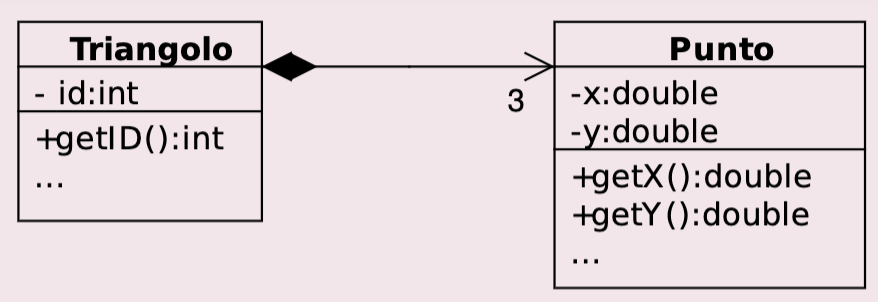
\includegraphics[width=0.6\linewidth]{assets/UML/class/class-2.png}}
    \hfill
    \subfloat[Object Diagram]{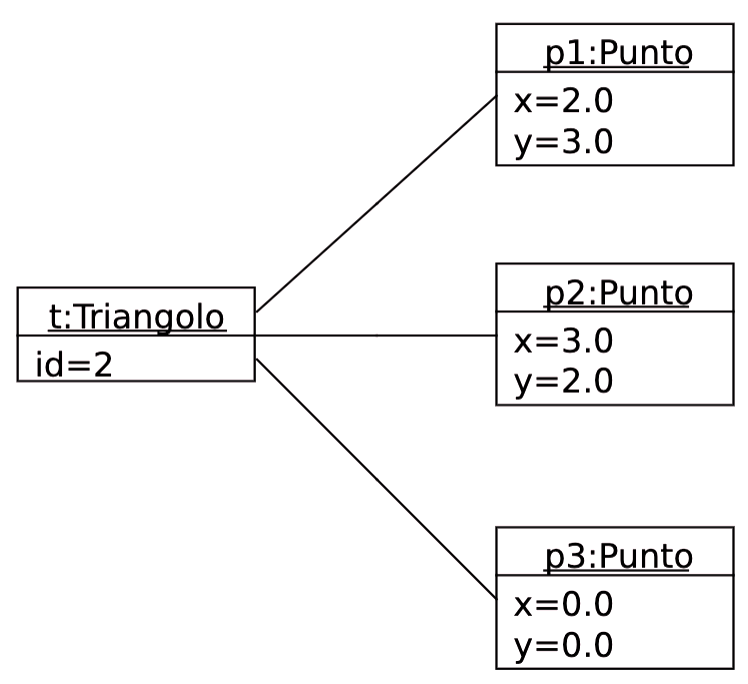
\includegraphics[width=0.3\linewidth]{assets/UML/object/object-1.png}}
    \caption{Differenze tra classi e oggetti in UML}
\end{figure}

\paragraph{Note} È possibile \textit{omettere degli attributi} oppure \textit{mostrare istanze di classi astratte}.

\paragraph{Relazioni} Nonostante il cambio di prospettiva dalle classi agli oggetti, le relazioni illustrate da un object diagram sono sempre di tipo \textit{statico}: il diagramma è una sorta di “fotografia congelata nel tempo”; mostra gli oggetti che costituiscono il sistema in un determinato momento.

\begin{figure}[h!]
    \centering
    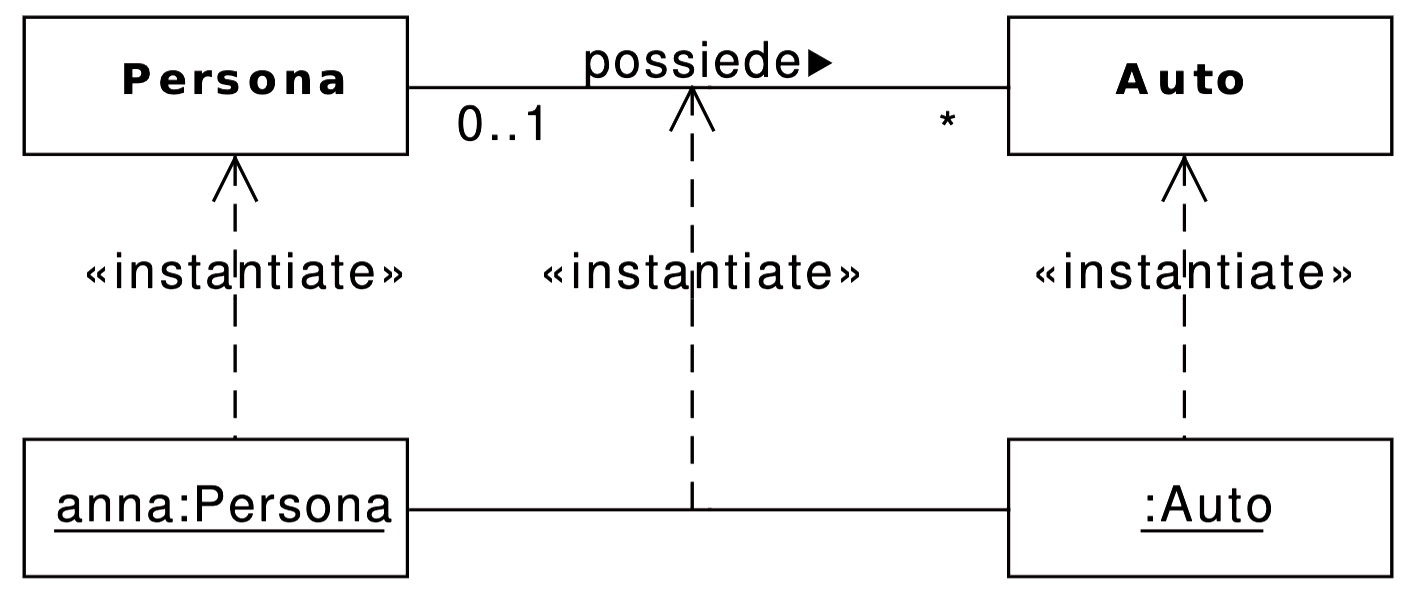
\includegraphics[width=0.75\linewidth]{assets/UML/object/object-2.png}
    \caption{La relazione di dipendenza $\langle$$\langle$instantiate$\rangle$$\rangle$ indica esplicitamente che gli oggetti sono istanze di classi ed il link è un'istanza della relazione \textit{possiede}.}
\end{figure}

\newpage